\documentclass[11pt, letterpaper, oneside]{article}
\usepackage{enumerate}
\usepackage{ calc }
\usepackage{ amssymb }
\usepackage{graphicx}

\begin{document}

\title{\textbf{CMCS 818J Project Final Report}}
\author{Behzad Koosha, Christopher Imbriano}

\maketitle

\section{Abstract}

	In this report we will be describing a scheme for achieving a streaming authenticated data structure (SADS) proposed by Papamanthou and 
	Shi \cite{sads}. The goal of this project is twofold. First, we will be implementing an example of this data
	structure and second, we will be building an application using the SADS primitive. 


\section{Introduction}

	In the verifiable computation (VC) problem, a client wishes to compute a complex
	function f on an input x. The client does not trust the server and therefore, would like to
	be able to verify the correctness of the computation without investing too much resources.
	The increasing use of distributed computing over the internet also makes strong servers more commonly 
	available. The growth of outsourcable computation in the form of cloud computing has attracted a renewed
	interest in the VC problem, and a considerable amount of research has been devoted to these problems \cite{evsc}.\\ 
	
	The introduced scheme, Streaming Authenticated Data Structure (SADS), does not require any interaction between the client and the server while the stream is observed.
	Three important properties are obtained using this scheme :
	\begin{enumerate}[a.]
	\item Independence of prover and verifier : the prover and the verifier update their status independently and with no interaction.
	\item Efficiency : It can be shown that an exponential improvement for many commonly queries in the prover's running time can be achieved.
	\item Expressiveness : a wide range of queries such as membership/ non-membership, successor, range search and frequencies can be supported using this scheme.
	\end{enumerate} 
	
	The ultimate goal of the proposed scheme is to build secure protocols that enable the verification of computation
	that is performed by an untrusted resource.\\
		
	The rest of this paper is organized as follows. We will be describing streaming authenticated data structure 
	goals. Some recent research in streaming verifiable computation will be discussed. We then describe the 
	homomorphic property used in the the SADS scheme. Some definitions will be presented in the following section.
	We present significant features of our implementation afterwards followed by presenting the performance of 
	our investigation. Finally, we conclude our paper by providing some future plans.\\
	
	\section{A Lattice-based Hash Tree Model}
	
	The bottomline for the proposed scheme uses Merkle tree structure using a hash function that has the homomorphic
	property. A way to map the outputs to the input domain considers \textit{labels} and allocates the root digest as
	the sum of well defined functions, nameley, \textit{partial digests} applied to the leaves of the Merkle tree.
	This will ease for the felxibility and efficiency in streaming update for the verifier and prover. \\
	
	Each node in the tree has a label $\lambda$ and a digest \textit{d}, where a node's digest
	could be computed uniquely from its label. Given two children labels, the digest of the parent can be 
	calculated. Figure one represents this property. The labels are denoted by circles and digests are 
	represented with squares. \\
	
        \begin{figure}[h]
        \centering
        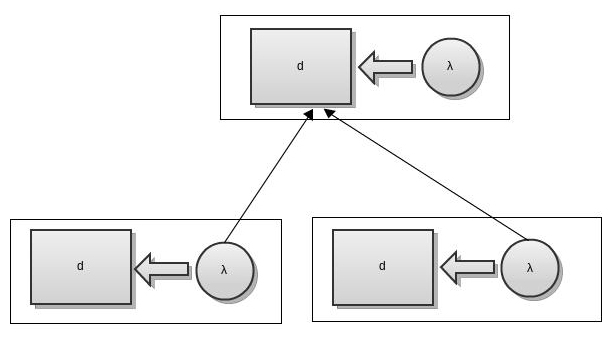
\includegraphics[width=100mm]{./images/label_digest.jpg}
        \caption[]{Labels and Digests}
        \end{figure}

	
	As an example, if the set of elements contains the nodes {1,4,6,7} the digest of the hash root of the tree 
	could be expressed as : \textit{D}(1)+\textit{D}(4)+\textit{D}(6)+\textit{D}(7)
        where \textit{D}(x) is the partial digest of the root with respect to x. \\
	
	The hash function is calculated as follows. Given a security parameter \textit{k}, $\textit{n} = 
	poly(\textit{k})$ and $\textit{q} $, $\textit{$\mu$}$, $\textit{$\beta$}$ outputed parameteres by the SADS 
	algorithm, $\textbf{L}, \textbf{R} \in Z $ two (k $\times$ m) random uniform matrices in \textit{mod q}, the 
	hashed function is defined as h(x,y)= $\textbf{L}$.x + $\textbf{R}$.y mod q. \\ 
	
	\section{Properties of Digests and Labels}
	
	\begin{enumerate}
	\item Having a label of a node, its digest can be computed (not necessarily the other way around)
	\item Having the labels of the two children nodes, using the hash functions, the digest of the parent
	      could be computed.
	\end{enumerate}
	
	\section{Prover}
	
	The proof of leaf node \textit{i} consists of: 
	\begin{enumerate}
	 \item the labels of nodes from \textit{i} to the root
	 \item the sibling nodes to that path
	\end{enumerate}
	
	In figure two, the labels are presented in green (path to the root) while the sibling
	nodes to that path are colored in blue. 

	\begin{figure}[h]
        \centering
        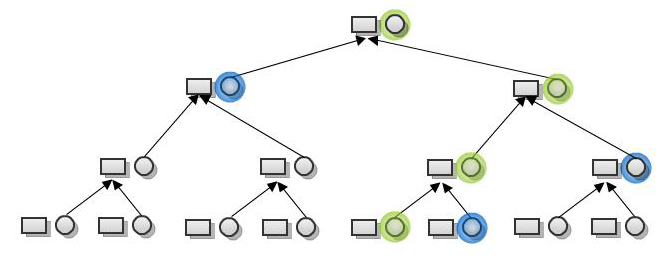
\includegraphics[width=100mm]{./images/8.jpg}
        \caption[]{Prover}
        \end{figure}
	
	
	\section{Verifier}
	
	The verifier computes the digest for every node on the path from \textit{i} to the root in two ways, and checks
	if they are consistent :
	
	\begin{enumerate}
	 \item using the \textit{labels} of its children
	 \item from the \textit{label} of the node itself
	\end{enumerate}

	
	\section{Our Approach}
	
	The description of the SADS scheme reads much like a protocol, focusing on the behaviour of each of the prover and verifier during a streaming phase and a query phase.
	Before tackling the problem at the protocol level however, we must first implement the basic data structures each of the verifier and prover will need to perform their roles.
	This will be our starting point.

	The road map for this project is as follows:
	\begin{enumerate}
	\item Implement underlying Merkle tree with homomorphic hash function
	\item Implement the SADS scheme
	\item Develop proof-of-concept application using the SADS scheme implementation
	\end{enumerate}

	\subsection{Underlying Data Structures}

	A crucial component of the SADS algorithm relies on matrix multiplication, a relatively expensive computational operation.
	When formulating our plan of action for this project, we were recommended a few linear algebra libraries, which will be discussed in a later section.
	While we recognize the importance of fast matrix operations and parallelism for production quality code, we thought that the added complexity, as well as unknowns with respect to implementation details, would be prohibitive.
	Instead, we've decided to use an interpreted language and the simple matrix operations that come with the standard libraries to start.

	Our language of choice for this first stage of the project is Ruby. Ruby has a number of advantages including:

	\begin{enumerate}
	\item Built-in support of matrix and vector operations
	\item Vibrant developer community that supports both new and experienced developers through learning resources, tool development, etc...
	\item Ability to write compiled extensions in C
	\item Numeric and visualization library, SciRuby
	\end{enumerate}

	\subsection{SADS Scheme}

	Once the underlying data structure is complete, the SADS scheme will use it as a primitive.
	Though one of the scheme's strengths is the independence of the prover and verifier during the streaming setting, the two parties will necessarily need to communicate during the query phase.
	Additionally, there may be communication between the two parties to initiate the streaming setting.
	For these reasons, we anticipate creating an application which will require network communication as it will likely be the case that the verifier and prover are not collocated.

	%We have a few frameworks in mind for this task.
	%Two of our options at the moment are EventMachine and Node.js.
	%Node.js is a "platform for building fast, scalable network applications" and has been gaining popularity in the Ruby community. http://nodejs.org/
	%EventMachine is a "fast, simple event-processing library for Ruby programs."http://rubyeventmachine.com/

\section{ Benchmarking }
	
	The next stage of development is benchmarking to understand the performance of the implementation and to differentiate constraints resulting from particular design decisions from those arising from the schemes protocol itself.
	We will focus primarily on benchmarking the timing of important operations in the scheme as well as the memory footprint of the implementations largest data structures.
	
	We ran some preliminary calculations to ballpark the size of L and R the public key of the SADS scheme.
	Recall, L and R are two matrices having elements in Z q, where q is derived from the security parameter k and the upper bound on the size of the stream, n.
	So a rough estimate of the size of L and R would be the size of the matrices, (ie. the number of elements) multiplied by the amount of space required for each element.
	Below is a table of these preliminary calculations.
	
	\begin{table}[h]
	\centering
		\begin{tabular}{ c | c | c | c}
		k & n & Matrix dim & Footprint\\ \hline
		500&10&500 x 1500&2MB\\
		500&100&500 x 1500&2MB\\
		500&1000&500 x 1500&2MB\\
		500&10000&500 x 1500&2MB\\
		500&100000&500 x 1500&3MB\\
		500&1000000&500 x 1500&3MB\\
		500&10000000&500 x 1500&4MB\\
		500&100000000&500 x 1500&4MB\\
		
		\end{tabular}
	\caption{ Estimation of public key size.  Constant security parameter, varying stream size upper bound }
	\label{tab:pub-key_n}
	\end{table}
	
	\begin{table}[h]
	\centering
	
		\begin{tabular} { c | c | c | c}
		
		k & n & Matrix dim & Footprint\\ \hline
		1000&100000&1000 x 3000&14MB\\
		10000&100000&10000 x 30000&1716MB\\
		100000&100000&100000 x 300000&171661MB\\
		1000000&100000&1000000 x 3000000&20027160MB\\
		10000000&100000&10000000 x 30000000&2288818359MB\\	
		\end{tabular}
	
	\caption{Estimation of public key size.  Constant stream size upper bound , varying security parameter } 
	\label{tab:pub-key_k}
	\end{table}
	
	The estimated memory footprint of the public key matrices grows rapidly with an increasing security parameter, but slowly with increasing stream size.
	The reason for this is that the scheme calls for matrices of size k x k log q.
	The matrix size grows faster than k SQUARED because q also depends on k.
	Fortunately, the current proposal is to pick a security parameter "large enough", say 500, and not to vary k over time.
	
	Future benchmarking efforts will also measure the memory footprint of the prover over time, and the size of a proof for varying parameter sizes.
	Additionally, we will benchmark the time required to perform the following tasks:
	
	\begin{itemize}
	\item Update prover state	
	\item Proof generation
	\item Update verifier state
	\item Proof verification
	\item Matrix multiplication using built-in Ruby implementation
	\item Matrix multiplication using optimized libraries
	\end{itemize}
	
	
	
\section{Looking Forward}

	\subsection{Production Quality Libraries}
	It is yet to be seen whether the existing Ruby matrix libraries, either the built in or SciRuby, 
	will be sufficiently efficient for the needs of the SADS scheme. That's not to say the current 
	choices of technologies will not produce production quality code but, as mentioned earlier, we have
	been investigating some optimized libraries listed here.

	\begin{enumerate}
	\item \textbf{NTL 5.5.2} : A free software written in C++ providing data structures and algorithms for arbitrary length integers, for vectors, matrices and polynomials over the integers and over the finite fields and for arbitrary precision floating point arithmetic. \texttt{http://shoup.net/ntl/}
	\item \textbf{MAGMA V2.18} : The kernel of Magma contains implementations of many of the important concrete classes of structure in five fundamental branches of algebra, namely group theory, ring theory, field theory, module theory and the theory of algebras.
	In addition, certain families of structures from algebraic geometry and finite incidence geometry are included. \texttt{http://magma.maths.usyd.edu.au/}
	\end{enumerate}

	
	%\subsection{Semester Outlook}
		%While the ultimate goal of the project is to produce a proof-of-concept application which utilizes a SADS scheme, it is best to set manage expectations.
		%Our baseline target for this semester is to complete the first two layers described above, that is the underlying data structure and the SADS scheme primitive.
		%Having completed these two components, we can then establish time line during which the proof-of-concept application can be hashed out and developed.
		%We hope to leverage the Ruby and broader open-source community by packaging this application, or just the SADS scheme primitive, into a library for others to use and provide feedback.


%%%%%%%%%%%%%%%%%%%%%%%%%%%%%%%%%%%%%%%%%%%%%%%%%%%%%%%%%%%%%%%%%%%%%%%%

\begin{thebibliography}{9}
	\bibitem{sads} Elaine Shi, Charalampos Papamanthou \emph{Streaming Authenticated Data Structures}, Date Unknown
	\bibitem{evsc} B. Applebaum, Y. Ishai
and E. Kushilevitz \emph{From Secrecy to Soundness:
Efficient Verification via Secure Computation}
	\end{thebibliography}

\end{document}
